\documentclass[11pt]{article}

\usepackage{amsmath,amssymb,amsfonts}
\usepackage{dsfont}
\usepackage{listings}
\usepackage{xcolor}
\usepackage{graphicx}
\usepackage{bbm}
\usepackage{float}


\definecolor{codegreen}{rgb}{0,0.6,0}
\definecolor{codegray}{rgb}{0.5,0.5,0.5}
\definecolor{codepurple}{rgb}{0.58,0,0.82}
\definecolor{backcolour}{rgb}{0.95,0.95,0.92}
\lstdefinestyle{mystyle}{
    backgroundcolor=\color{backcolour},
    commentstyle=\color{codegreen},
    keywordstyle=\color{magenta},
    numberstyle=\tiny\color{codegray},
    stringstyle=\color{codepurple},
    basicstyle=\ttfamily\footnotesize,
    breakatwhitespace=false,
    breaklines=true,
    captionpos=b,
    keepspaces=true,
    numbers=left,
    numbersep=5pt,
    showspaces=false,
    showstringspaces=false,
    showtabs=false,
    tabsize=2
}

\setlength{\topmargin}{-.5in} \setlength{\textheight}{9.25in}
\setlength{\oddsidemargin}{0in} \setlength{\textwidth}{6.8in}

%\newcommand*{\SOLVE}{}%

\renewcommand{\vec}[1]{\mbox{\boldmath$#1$}}
\newcommand{\mm}[1]{\mathbf{#1}}

\newcounter{ProblemNum}
\newcounter{SubProblemNum}[ProblemNum]

\renewcommand{\theProblemNum}{\arabic{ProblemNum}}
\renewcommand{\theSubProblemNum}{\alph{SubProblemNum}}

\newcommand*{\anyproblem}[1]{\section*{#1}}
\newcommand*{\problem}[1]{\stepcounter{ProblemNum} %
   \anyproblem{Problem \theProblemNum \; (#1 points)}}
\newcommand*{\soln}[1]{\subsection*{#1}}
\newcommand*{\solution}{\soln{Solution}}
\newenvironment{solutions}
  {\section[Solution]{\textcolor{red}{Solution}}\color{red}}
  {\normalcolor}
\renewcommand*{\part}{\stepcounter{SubProblemNum} %
  \soln{Part (\theSubProblemNum)}}
\renewcommand{\theenumi}{(\alph{enumi})}
\renewcommand{\labelenumi}{\theenumi}
\renewcommand{\theenumii}{\roman{enumii}}
\let\endsection\relax
\let\endsubsection\relax

\graphicspath{
{.}
}
\lstset{style=mystyle}

\begin{document}

\Large
\noindent{\bf CS4851/6851 IDL: Homework 1 \hfill \today}
\medskip\hrule

\vspace{20pt}

Note: All coding problems are to be implemented in a single jupyter notebook.

Note: this is the distribution of questions:
\begin{enumerate}
  \item Question 1 to Question 8: Required for everyone.
  \item Question 9 - Question 10: Required only for Graduate Students
  \item Question 11 - Question 12: Bonus marks
\end{enumerate}

\problem{5} What is the difference between Root Mean Squared Error (RMSE) and Mean Squared Error(MSE). Describe the context in which they will be most useful? Which of these losses penalizes large differences between the predicted and expected results and why?

\problem{5} Which of the following statements is true about the relationship between features and dataset sizes? Choose one of the following and explain the chosen answer
\begin{enumerate}
  \item When training a model, as you add more features to the dataset, you often need to increase the dataset's size to ensure the model learns reliably.
  \item When training a model, adding more features to the dataset increases the amount of information you can extract from the dataset. This allows you to use smaller datasets to train the model and still achieve good generalization performances from the training data.
  \item When training a learning algorithm, as you decrease the number of features in the dataset, you need to increase the training sample size to make up the difference.
  \item When training a learning algorithm, the number of features in your dataset is entirely dependent on the amount of information you can extract from the dataset.
\end{enumerate}

\problem{4} You are building a deep learning model and after $X$ epochs you see that the training loss is decreasing, while your validation loss is either constant or increasing. What would be the most likely cause of this and suggestion to rectify it
\begin{enumerate}
  \item Learning rate is too high
  \item Gradient descent does not converge
  \item Insufficient training data size
  \item Gradient descent is stuck in a local minimum
\end{enumerate}

\problem{4}  Perceptron
\begin{enumerate}
  \item is a linear classifier. A. True  B. False
  \item and cannot be trained on linearly unseperable data. A. True  B. False
\end{enumerate}

\problem{4}  Logistic Regression
\begin{enumerate}
  \item is a linear classifier. A. True  B. False
  \item and always has a unique solution A. True  B. False
\end{enumerate}


\problem{10} Which of the following is true, given the optimal learning rate?
\begin{enumerate}
  \item Batch gradient descent is always guaranteed to converge to the global optimum of a loss function.
  \item Stochastic gradient descent is always guaranteed to converge to the global optimum of a loss function.
  \item For convex loss functions (i.e. with a bowl
    shape\footnote{More formally $f$ is convex on $[a,b]$ if $\forall
      \vec{x}_1, \vec{x}_2 \in [a,b]$ if $f(\lambda\vec{x}_1 +
      (1-\lambda)\vec{x}_2) \le \lambda f(\vec{x}_1) + (1-\lambda) f(\vec{x}_2)$}), batch gradient descent is guaranteed to eventually converge to the global optimum while stochastic gradient descent is not.
  \item For convex loss functions (i.e. with a bowl shape), stochastic gradient descent is guaranteed to eventually converge to the global optimum while batch gradient descent is not.
  \item For convex loss functions (i.e. with a bowl shape), both stochastic gradient descent and batch gradient descent will eventually converge to the global optimum.
  \item For convex loss functions (i.e. with a bowl shape), neither stochastic gradient ndescent nor batch gradient descent are guaranteed to converge to the global optimum.

\end{enumerate}

\problem{5}
Given the following data on a 2D plane :

\begin{center}
  \begin{tabular}{||r r ||}
   \hline
   x & y \\ [0.5ex]
   \hline\hline
   -1 & -2  \\
   \hline
   1 & -1  \\
   \hline
   2 & 3 \\[1ex]
   \hline
  \end{tabular}
  \end{center}

Fit a linear regression model to the data without the constant term: $y_{i} = \beta x_{i} + \epsilon_{i} $. Give an expression of the minimization problem for finding $\beta$, Show how to compute it's value and show the value

\problem{20}
Perform a polynomial fitting to compute a design matrix $X$ such that:

\begin{equation}
X_{ij} = y_{i}^j
\end{equation}

You should implement this \textbf{without a single for loop} by using vectorization and broadcast. Here ($1 \leq j \leq 50$)  and $y  = \{-20, -19.9, ..., 20\}$. Implement code that generates such a matrix.

\vspace{20pt}
\noindent\rule[0.5ex]{0.45\linewidth}{1pt} Bonus for undergraduates
beyond this line
\problem{15}
Is this a good idea to initialize parameters with zeros when training a logistic regression model? Explain your answer.

\problem{15}
As discussed in the class, the logistic regression likelihood simplifies to the following form:

\begin{align*}
  \mbox{cost}(f(x), y) &= -y \log(f(x)) - (1-y) \log(1-f(x))\\
  y & \in \{0, 1\} \mbox{ class label}
\end{align*}

What will happen when $y = 1$ and $f(x) = 1$? Will this work in actual implementations?

\vspace{20pt}
\noindent\rule[0.5ex]{0.7\linewidth}{1pt} Extra credit problems

\problem{extra credit 20} % 8
In the three examples of Figure~\ref{fig:decision_boundary}, find the perceptron weights $w_0, w_1, w_2$ for each of them.
The line that separates the two classes is given by the decision boundary that divied into positive and negative classes. (No calculations required, you can simply note the answer.)

\begin{figure}[H]
  \centering
  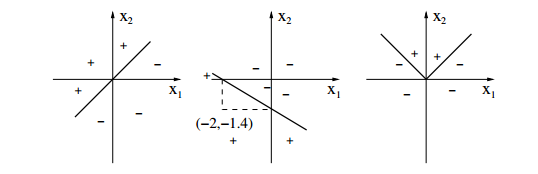
\includegraphics[width=0.8\textwidth]{homework_problem_1.png}
  \label{fig:decision_boundary}
  \caption{Binary class data and separating decision boundaries.
  }
\end{figure}

\problem{extra credit 20} % 8
Consider the evaluation of E as given below:

\begin{equation}
  E = g(x, y, z) = \sigma(c(ax + by) + dz)
\end{equation}

Here $x, y, z$ are inputs and $a, b, c, d$ are parameters. $\sigma$ is logistic sigmoid function defined as:

\begin{equation}
  \sigma(z) = \frac{1}{1 + e^{-z}}
\end{equation}
Note that E is the function of $a,b,c,d$
Compute the partial derivative of E with respect to parameters $a, b, d$ i.e $\frac{\partial{E}}{\partial{a}}, \frac{\partial{E}}{\partial{b}}, \frac{\partial{E}}{\partial{d}}$
\end{document}
%%% Local Variables:
%%% mode: latex
%%% TeX-master: t
%%% End: